\documentclass[14pt, table]{beamer}
%\documentclass[14pt, table, handout]{beamer}
%\usetheme{Luebeck}
\usetheme{Malmoe}
%\usetheme{Pittsburgh}
%\usetheme{Rochester}
%\usetheme{metropolis}

\usecolortheme{spruce}
%\usecolortheme{beaver}

% Get rid of footer
\setbeamertemplate{navigation symbols}{}
\setbeamertemplate{footline}{}

% Speaker notes
%\setbeameroption{show only notes}
%\setbeameroption{show notes}
%\setbeameroption{show notes on second screen}
\setbeamerfont{note page}{size=\footnotesize}
\addtobeamertemplate{note page}{
	\setbeamerfont{itemize/enumerate subbody}{size=\footnotesize}}{}
	
% highlighting
\usepackage{graphicx}
\usepackage{soul}

% Graphics and such
\usepackage{booktabs}
\usepackage[RPvoltages]{circuitikz}
\ctikzset{logic ports=ieee,logic ports/scale=1}

\usetikzlibrary{decorations.pathmorphing}
\usetikzlibrary{calc, positioning}
\usetikzlibrary{shapes.arrows, fadings}

\newcommand{\bigkey}[1] {
	\draw (#1) ++ (20:.5) coordinate (top) arc(20:340:.5) coordinate (bottom);
	\draw (#1) ++ (-.2,0) circle (.1);
	\draw (#1) ++ (.5,.1) -- ++ (1,0);
	\draw (top) -- ++(1.25,0)
	coordinate (tmp) -- ($(#1 -| tmp) + (.15,0)$)
	coordinate (tip);
	\draw [decorate, decoration={
		zigzag,
		segment length=10,
		amplitude=2.5,
		pre length = 5.57, % centers zigzag
		post length = 0
	}] (bottom) -- ++(1.25,0) coordinate (tmp);
	\draw (tmp) -- (tip);
}

\newcommand{\littlekey}[2] {
	\draw (#1)++(-.4,0) coordinate (center);
	\draw (center) node[] {\tiny{#2}};
	\draw (center)++ (20:.3) coordinate (top) arc(20:340:.3) coordinate (bottom);
	\draw (center)++ (-.2,0) circle (.05);
	%\draw (center)++ (.5,.1) -- ++ (.75,0);
	\draw (top) -- ++(.7,0)
	coordinate (tmp) -- ($(#1 -| tmp) + (.15,0)$)
	coordinate (tip);
	\draw [decorate, decoration={
		zigzag,
		segment length=5,
		amplitude=1,
		pre length = 2.5, % centers zigzag
		post length = 0
	}] (bottom) -- ++(.7,0) coordinate (tmp);
	\draw (tmp) -- (tip);
}

\newcommand{\lockshape}[2]{
	\draw (#1) ++ (-.7,.7) node [below right] {\footnotesize{#2}};
	\draw[thick] (#1) ++ (-60:.1) coordinate (right)
	arc (-60:240:.1)
	-- ++ (0,-.2) -| (right);
	\node[rectangle, draw, thick, minimum size=30] at (#1) (lastBox) {};
	%\draw (#1) ++ (-.7,.7) rectangle ++(1.4,-1.4);
}

\newcommand{\examplecircuit} {
	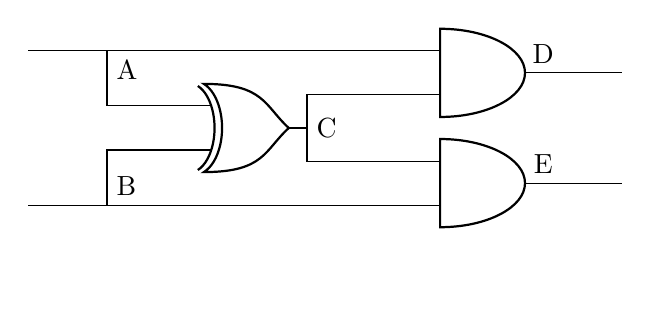
\begin{tikzpicture}
		\node[xor port] (xor)  at (0, 0){};
		\node[and port] (andA) at (3, .7){};
		\node[and port] (andB) at (3,-.7){};
		\draw (andA.in 1)  -- ++(-5, 0)
		      (andB.in 2)  -- ++(-5, 0)
		      (xor.in 1)   -| ++(-1, .7) node [below right] {A}
		      (xor.in 2)   -| ++(-1,-.7) node [above right] {B}
		      (andA.in 2)  -| (xor.out)  node [      right] {C}
		      (andB.in 1)  -| (xor.out)
		      (andA.out) node [above] {D} -- ++( 1, 0)
		      (andB.out) node [above] {E} -- ++( 1, 0)
		      (0,-2); % force a bit of padding
	\end{tikzpicture}
}


\title{Mobile Cryptographic Coprocessor for Privacy-Preserving Two-Party Computation}
\subtitle{Yao's Garbled Circuits}
\author{Gabriel Kulp}
\date{May 28, 2021}
\institute{kulpga@oregonstate.edu}

\begin{document}
\maketitle{}
\note{
Hi! I designed a hardware addon that you can connect to a smartphone to help it do some crazy cryptography faster. Specifically, it evaluates garbled circuits, which are a way to perform computations on different people private data while keeping it private.

}

\begin{frame}
	\centering
	\Huge
	Algorithm
	\color{gray}
	\normalsize
	\vspace{5mm}
	
	\pause
	Software
	
	\pause
	\vspace{4mm}
	Hardware
\end{frame}
\note{
I will start my presentation with a lot of background information about the algorithm I devoted Fall term to learning about. (adv) Then we'll talk about software considerations and design decisions to implement that algorithm, which was basically my Winter term, (adv) and then I'll move into the hardware design, which I worked on this Spring term.

The algorithm I'm going to talk about performs a multi-party computation.

}

\begin{frame}{What is Multi-Party Computation?}
	\begin{itemize}[<+->]
		\item MPC = multi-party computation
		\item Interactive cryptographic protocol
		\item Compute on private inputs
		\item Trust nobody
	\end{itemize}
\end{frame}
\note{
Multi-party computation, or MPC, is a field of cryptography dealing with the design of (advance) of a protocol where some people send cryptographic messages back and forth. (advance) The point of an MPC protocol is to compute the output of some function on private inputs held by each party, but without those parties needing to share their inputs. If you could trust someone to do the computation and keep everyone's inputs secret, then we wouldn't need the cryptography part. (advance) MPC removes the need to trust other parties, but at the cost of lots of math and network traffic.

}


\begin{frame}{Motivation}
	\begin{block}{Who has more money?}
		\begin{itemize}
			\item Millionaires at a party
			\item They don't want to share
			\item No trusted parties
		\end{itemize}
	\end{block}
	\pause
	\begin{block}{Sharing student data}
		\begin{itemize}
			\item Dip in Estonian CS degrees
			\item Tech companies poaching?
			\item Data privacy laws
		\end{itemize}
	\end{block}
\end{frame}
\note{
Let's start with why anybody cares about this.

The classic example is that there are two millionaires at a party that want to find out who has more money, but they don't want to say how much money they have. They could whisper in the butler's ear, but he might give tell someone later or give the wrong answer, so they'd rather not trust anybody.

(advance) A real example from Estonia is that a university wanted to ask some tech companies if there was a correlation that would suggest students were getting hired out of college before finishing their degrees. Estonia has strong privacy laws, though, and sharing that kind of student and employee data would be illegal. They were able to execute a multi-party computation to calculate the correlation of their private datasets and learn something that no party could legally have computed on their own.

There are many other examples like these. In the States we have HIPPAA and FERPA to protect healthcare and student records, but there might be some really good data science we could do if institutions could freely share this information. One solution is to use MPC to perform computations on this data without actually sharing it in the clear.

If you're new to cryptography or haven't heard of Garbled Circuits, this probably sounds like black magic. I'm hoping you can come away from my presentation feeling like it's a little less mysterious.

}


\begin{frame}[t]{Basic Concepts}
	\begin{columns}
		\begin{column}{.7\textwidth}
			\begin{block}{Boolean Circuits}
				\begin{itemize}
					\item AND and XOR
					\item Connected by wires
					\item Performs computation
				\end{itemize}
			\end{block}
			\pause
			\begin{block}{Symmetric-Key Encryption}
				\begin{itemize}
					\item Advanced Encryption Standard
					\item Keys and locks
				\end{itemize}
			\end{block}

			\pause
			Oblivious transfers covered later
		\end{column}
		\begin{column}{.3\textwidth}
			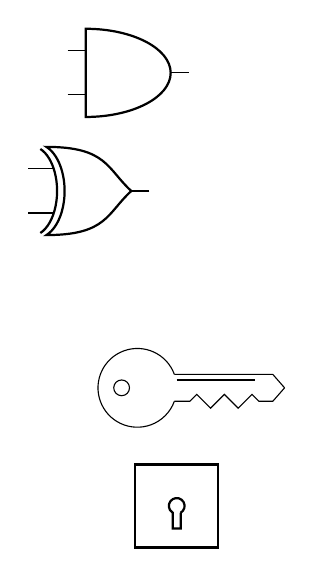
\begin{tikzpicture}
				\pause[0]
				\node[and port] (and) at (.5, 1.5){};
				\node[xor port] (xor) at (0, 0){};
				\draw (0,2) (0,-4.6);
				\only<2->{
					\bigkey{0,-2.5};
					\lockshape{.5,-4}{}
				}
			\end{tikzpicture}
		\end{column}
	\end{columns}
\end{frame}
\note{
To start describing how this works, I'm going to first explain boolean circuits. A boolean circuit is a bunch of logic gates like AND and XOR connected together by wires. Boolean circuits can compute any math expression, but it might take a lot of gates.

(adv) After I go into boolean circuits, I'll talk about symmetric encryption. The Advanced Encryption Standard is a well-studied encryption algorithm, but its specifics don't matter quite yet, so it's fine to think about a cryptographic key as a literal key and a ciphertext as a locked box. Without the key, you don't know what's in the box. In this case, you need the key to open OR close the box.

(adv) There's another basic concept that MPC builds with called an Oblivious Transfer, but I'll cover that when we get there.

}


\begin{frame}{What's Garbling?}
	\centering
	\newcommand*\changingline{}
	\newcommand*\changingbox{draw}
	\only<2->{\renewcommand{\changingline}{[dashed, black!10!white]}}
	\only<2->{\renewcommand{\changingbox}{black!10!white}}
	\begin{tikzpicture}[
		clearbox/.style={rectangle, draw, thick, minimum size=10mm},
		clearIO/.style={rectangle, thick, minimum size=10mm},
		garbledbox/.style={rectangle, draw, thick, minimum size=15mm,align=center},
		garbledIO/.style={rectangle, thick, minimum size=15mm, align=center},
		->,  % makes the edges directed
		>=stealth, % makes the arrow heads bold
		line width=.5mm,
		node distance=2cm,
		]
		\node[clearIO] (i)  {Input};
		\node[clearbox, right=of i,\changingbox] (c) {Circuit};
		\node[clearIO, right=of c] (o) {Output};
		\draw \changingline{} (i) -- (c);
		\draw \changingline{} (c) -- (o);
		\pause
		
		\node[garbledbox, below=of c] (gc) {Garbled \\ Circuit};
		
		\node at ($(c)+(0,-1.33cm)$) [
			top color=black!10!white,
			bottom color=red,
			single arrow,
			minimum height=2cm,
			minimum width=10mm,
			inner sep=0mm,
			single arrow head extend=.1mm,
			rotate=270, single arrow
		] {};

		\pause
		\node[garbledIO, below=of i] (gi) {Garbled \\ Input};
		\draw[red] (i)  -- (gi);
		\pause
		\draw[blue] (gi) -- (gc);
		\pause
		\node[garbledIO, below=of o] (go) {Garbled \\ Output};
		\draw[blue] (gc) -- (go);
		\pause
		\draw[red] (go) -- (o);

	\end{tikzpicture}
\end{frame}
\note{
Evaluating a circuit with the Garbled Circuits protocol requires starting with a normal circuit. Here's what that looks like. An input is converted to something you can put into the circuit on the left side, then the input is propagated through the circuit, and the output comes out the right side.

The garbled circuits protocol is split into two roles. There's the garbler, who I'll call Alice and draw with red, and the evaluator, who I'll call Bob and draw with blue. Alice has to first garble the circuit. (advance) Obviously you don't know what that means yet, but for now it's just a secret transformation. Next, (advance) she works with Bob, who doesn't know the secret transformation, to turn the circuit's input into a garbled input. Alice and Bob both supply part of the circuits input. Bob then puts this input into the garbled circuit (advance), and follows the calculation blindly, since he doesn't know the transformation, to yield the (advance) garbled output. Finally, (advance), Alice helps him turn the garbled output back into the real output, since she's the only one who knows exactly how the circuit was garbled.	

Don't get too scared by this picture just yet. I'm just showing you a roadmap for now and then I'll show the picture again once I've explained what all the pieces mean.

}


\begin{frame}{Boolean Circuit}
	\centering
	\examplecircuit
	\pause
	\begin{columns}
		\begin{column}{.3\textwidth}
			\centering
			\begin{tabular}{c c | c}
				A & B & C \\
				\midrule
				0 & 0 & 0 \\
				0 & 1 & 1 \\
				1 & 0 & 1 \\
				1 & 1 & 0 \\
			\end{tabular}
		\end{column}
		\pause
		\begin{column}{.3\textwidth}
			\centering
			\begin{tabular}{c c | c}
				A & C & D \\
				\midrule
				0 & 0 & 0 \\
				0 & 1 & 0 \\
				1 & 0 & 0 \\
				1 & 1 & 1 \\
			\end{tabular}
		\end{column}
		\pause
		\begin{column}{.3\textwidth}
			\centering
			\begin{tabular}{c c | c}
				B & C & E \\
				\midrule
				0 & 0 & 0 \\
				0 & 1 & 0 \\
				1 & 0 & 0 \\
				1 & 1 & 1 \\
			\end{tabular}
		\end{column}
	\end{columns}
\end{frame}
\note{
Let's start with a closer look at what exactly a circuit is.

Here's an example of a simple boolean circuit. The input wires are on the left side labeled A and B, the output wires are on the right, D and E. All the logic flows from left to right, with no outputs looping back to the left. Gates are referred to by the ID of their output, so the one on the left is called Gate C.

(adv) Gate C is an XOR gate and this table describes how it works. The two input wires on the left of the gate are the A and B columns, and the output is C. Each row of the table shows the output for one combination of inputs.

(advance) And here's a table for Gate D, an AND gate, (adv) and here's the same table for Gate E, which is also an AND gate.

(draw on slides) Let's walk through this just to be very explicit. Let's assign a label of 0 to wire A and a label of 1 to wire B to form our inputs. We can't figure out the outputs D and E yet, since those gates rely on C which we don't have.

We can figure out what label to put on wire C by looking at the table for gate C on the left. From the second row, we can see that the label on wire C should be 1.

Now we know everything required to evaluate the last two gates and find the output of the computation.

(clear drawings) Now I'm gonna change things up a bit. You might be used to thinking of AND as an operation that combines values like True or False and returns another value that's either True or False. But actully, there's no need!

}


\begin{frame}{Boolean Circuit (still)}
	\centering
	\examplecircuit
	\begin{columns}
		\begin{column}{.3\textwidth}
			\centering
			\begin{tabular}{c c | c}
				A      & B        & C \\
				\midrule
				$\psi$ & $\phi  $ & $\cap$ \\
				$\psi$ & $\delta$ & $\Leftrightarrow$ \\
				$\pi $ & $\phi  $ & $\Leftrightarrow$ \\
				$\pi $ & $\delta$ & $\cap$ \\
			\end{tabular}
		\end{column}
		\pause
		\newcommand*\rhl{} % row highlight
		\only<4->{\renewcommand{\rhl}{\rowcolor{yellow}}}
		\begin{column}{.3\textwidth}
			\centering
			\begin{tabular}{c c | c}
				A      & C                 & D \\
				\midrule
				$\psi$ & $\cap$            & $\forall$ \\
				$\psi$ & $\Leftrightarrow$ & $\forall$ \\
				$\pi $ & $\cap$            & $\forall$ \\
				\rhl$\pi $ & $\Leftrightarrow$ & $\varnothing$ \\
			\end{tabular}
		\end{column}
		\pause
		\begin{column}{.3\textwidth}
			\centering
			\begin{tabular}{c c | c}
				B        & C                 & E \\
				\midrule
				$\phi  $ & $\cap$            & $\geqq$ \\
				$\phi  $ & $\Leftrightarrow$ & $\geqq$ \\
				$\delta$ & $\cap$            & $\geqq$ \\
				$\delta$ & $\Leftrightarrow$ & $\pitchfork$ \\
			\end{tabular}
		\end{column}
	\end{columns}
	\pause
\end{frame}
\note{
Here I've replaced the 0 and 1 values with arbitrary symbols. Pi and Phi and arrows don't mean anything on their own. They still describe a binary operation, though.

Of course if the C wire is going to be labeled with either a cap or arrows, then gates D and E need to be expecting those kinds of labels as inputs.

(adv) So this table shouldn't be a surprise. The possible labels on the A wire are still Psi and Pi, and we already knew from the previous truth table that the possible labels on the C wire are cap and arrows.

(adv) And this table really shouldn't be a surprise.

(draw) So when we choose our inputs, we choose between the options available on the table. So let's choose Psi and delta as the labels for A and B, and then look at the table to figure out the label for C. Looks like we match the second row, so that means we put arrows on wire C.

Then that's the second row for gate D, and the pitchfork for table E.

This is going to be useful for evaluating a circuit blindly, but there's actually another two steps before we can call this circuit properly garbled.

Right now someone can figure out from this row (adv) that Pi and arrows must both mean True. You can tell this for two reasons. First, the tables are always in the same order, so the last entry always means both inputs are True. Second, even though the output symbols are arbitrary, you can still tell that there are three upside-down A's and only one slashed circle. Since this is an AND gate, you only get a different output when both inputs are True, so the different output on the bottom row must be when both inputs are True.

You can solve the first problem by permuting the rows randomly, but the second problem requires some new material.

}

\begin{frame}{Symmetric-Key Encryption}
	\begin{columns}
		\begin{column}{.4\textwidth}
			\centering
			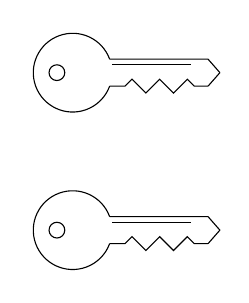
\begin{tikzpicture}
				\bigkey{0,1}
				\bigkey{0,-1}
			\end{tikzpicture}
		\end{column}
		\begin{column}{.6\textwidth}
			\begin{itemize}
				\item Each lock has one key
				\item Each box has two locks
				\item Put anything inside box
			\end{itemize}
		\end{column}
	\end{columns}
\end{frame}
\note{
I need to very briefly cover encryption how we're going to use it. Everything will be encrypted with two keys, so you can picture a box that has two locks on it, and you need both keys to open it. You can put whatever you want inside the box of course, but this is what makes things *really* interesting.

}


\newcommand{\enc}[3]{\(\textrm{enc}(\{#1, #2\}, #3)\)}
\begin{frame}{Garbling a Gate}
	\centering
	\begin{tabular}{c c | l}
		A      & C                 & \multicolumn{1}{c}{D} \\
		\midrule
		$\psi$ & $\cap$            & \enc{\psi}{\cap\hspace{1.5mm}}{\forall} \\
		$\psi$ & $\Leftrightarrow$ & \enc{\psi}{\Leftrightarrow}{\forall} \\
		$\pi $ & $\cap$            & \enc{\pi }{\cap\hspace{1.8mm}}{\forall} \\
		$\pi $ & $\Leftrightarrow$ & \enc{\pi }{\Leftrightarrow}{\varnothing}
	\end{tabular}
	\color{white} % just for spacing to align with the next one
	\[\textrm{dec}(\{\pi, \cup\}, 1101110001) = \forall\]
\end{frame}
\note{
Alright, so here's the breakthrough. What if we encrypt the output to each row? And we'll use the wire labels themselves as the key! Bob, who's evaluating the circuit, will only know the current label on wire A, called the "active" label; he doesn't know what the other label could be since it's arbitrary. Same with wire C.

}

\begin{frame}{Garbling a Gate}
	\centering
	\begin{tabular}{c c | c}
		A                   & C                              & D \\
		\midrule
		\color{gray} $\psi$ & \color{gray} $\cap$            & $0111010110$ \\
		\color{gray} $\psi$ & \color{gray} $\Leftrightarrow$ & $0010111011$ \\
		\color{gray} $\pi $ & \color{gray} $\cap$            & $1101110001$ \\
		\color{gray} $\pi $ & \color{gray} $\Leftrightarrow$ & $0010001100$
	\end{tabular}
	\color{white} % just for spacing to align with the next one
	\[\textrm{dec}(\{\pi, \cup\}, 1101110001) = \forall\]
\end{frame}
\note{
Also, Bob can't actually see all the symbols on the input side of the table, and he can't see inside the encrypted values, either; they look random until decrypted.

There's still the problem where Bob can figure out too much from the order of the table. To solve this, we do one last operation and permute the table randomly.

}

\begin{frame}{Garbling a Gate}
	\newcommand*\rhl{} % row highlight
	\only<2->{\renewcommand{\rhl}{\rowcolor{yellow}}}
	\centering
	\begin{tabular}{c c | c}
		A                   & C                              & D \\
		\midrule
		\rhl\color{gray}$\pi$&\color{gray} $\cap$            & $1101110001$ \\
		\color{gray} $\psi$ & \color{gray} $\cap$            & $0111010110$ \\
		\color{gray} $\psi$ & \color{gray} $\Leftrightarrow$ & $0010111011$ \\
		\color{gray} $\pi $ & \color{gray} $\Leftrightarrow$ & $0010001100$
	\end{tabular}
	\pause
	\[\textrm{dec}(\{\pi, \cup\}, 1101110001) = \forall\]
\end{frame}
\note{
So if Bob has Pi on wire A and Cap on wire C, then the only entry he has a valid key for is this one (adv), which decrypts to the upside-down A. He doesn't know that the other options are Psi and arrows, and he doesn't know that the other output is the slashed circle.

This means that Bob can take the inputs to the gate and figure out the output, but he doesn't learn anything about the semantic value of the arbitrary input or output labels. To be clear, Alice sets all this up and chooses the arbitrary labels and does the encryptions, so she knows exactly what's hiding in here.

If Alice had the inputs to evaluate the circuit, she would know Bob's inputs, which isn't allowed and defeats the whole purpose. So Bob needs to be the one to evaluate the circuit, since he can do it blindly. This of course requires Alice to set things up in such a way that Bob is actually blind. She does this by choosing arbitrary wire labels, encrypting the truth table outputs with the inputs as keys, and then randomly transposing the table.

}


\begin{frame}{What's Garbling?}
	\centering
	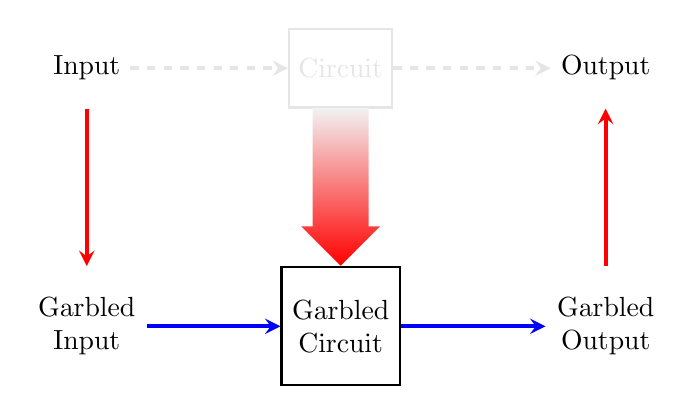
\begin{tikzpicture}[
		clearbox/.style={rectangle, draw, thick, minimum size=10mm},
		clearIO/.style={rectangle, thick, minimum size=10mm},
		garbledbox/.style={rectangle, draw, thick, minimum size=15mm,align=center},
		garbledIO/.style={rectangle, thick, minimum size=15mm, align=center},
		->,  % makes the edges directed
		>=stealth, % makes the arrow heads bold
		line width=.5mm,
		node distance=2cm,
		]
		\node[clearIO] (i)  {Input};
		\node[clearbox, right=of i, black!10!white] (c) {Circuit};
		\node[clearIO, right=of c] (o) {Output};
		\draw[dashed, black!10!white] (i) -- (c);
		\draw[dashed, black!10!white] (c) -- (o);
		\pause
		
		\node[garbledbox, below=of c] (gc) {Garbled \\ Circuit};
		
		\node at ($(c)+(0,-1.33cm)$) [
			top color=black!5!white,
			bottom color=red,
			single arrow,
			minimum height=2cm,
			minimum width=10mm,
			inner sep=0mm,
			single arrow head extend=.1mm,
			rotate=270, single arrow
		] {};

		\pause
		\node[garbledIO, below=of i] (gi) {Garbled \\ Input};
		\node[garbledIO, below=of o] (go) {Garbled \\ Output};
		\draw[red] (i)  -- (gi);
		\draw[red] (go) -- (o);

		\pause
		\draw[blue] (gi) -- (gc);
		\draw[blue] (gc) -- (go);

	\end{tikzpicture}
\end{frame}
\note{
Alright, now we can come back to this picture to see what's left. The whole goal here is to evaluate a function. In our case, we represent that function as a boolean circuit.

There are two roles: Alice is the garbler. (adv) She picks a secret translation that she can apply to the circuit, its inputs, and its outputs.

(adv) Bob doesn't know the translation, so he's free to do the computation without leaking any private information.

Perhaps you've noticed a problem, though. How can Bob get the circuit's input to start with? Let's say that Alice's input goes on Wire A and Bob's input goes on Wire B.

}

\begin{frame}{Inputs?}
	\begin{columns}
		\begin{column}{.5\textwidth}
			\centering
			\begin{tabular}{c c | c}
				A      & B        & C \\
				\midrule
				$\psi$ & $\phi  $ & $\cap$ \\
				$\psi$ & $\delta$ & $\Leftrightarrow$ \\
				$\pi $ & $\phi  $ & $\Leftrightarrow$ \\
				$\pi $ & $\delta$ & $\cap$ \\
			\end{tabular}
		\end{column}
		\begin{column}{.5\textwidth}
			\centering
			\begin{tabular}{c c c}
				Wire & True   & False \\
				\midrule
				A    & $\psi$ & $\pi$ \\
				B    & $\phi$ & $\delta$
			\end{tabular}
		\end{column}
	\end{columns}
\end{frame}
\note{
Here's a table from earlier on the left and Alice's arbitrary label choices on the right.

Alice chooses these arbitrary labels to correspond to True and False, and she makes these choices for every wire.

Bob's the one to actually evaluate the circuit, so he needs to know which inputs to use.

Alice can just give Bob the right key for her own input A, since Bob doesn't know what it means. Only Alice can see the table on the right, so if she knows that her input is False, she just gives Bob Pi and he doesn't know what it means. He can still plug it into the table blindly, though.

Alice can't give Bob both options for wire B, because then he would learn too much about the gates. He could try evaluating the circuit with both inputs and figure out more that what they agreed on. At the same time, Bob can't just ask Alice for whatever label corresponds to True, since then Alice would know Bob's input and the whole thing would be pointless.

}


\usetikzlibrary{arrows}
\begin{frame}{The Oblivious Transfer}
	\centering
	%\includegraphics[width=.8\textwidth]{ot.eps}
	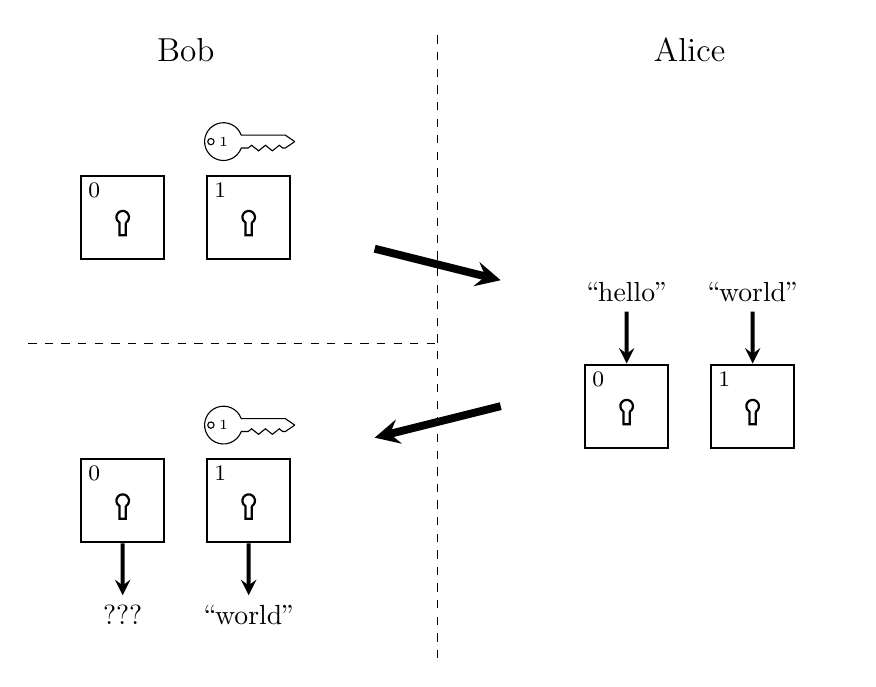
\begin{tikzpicture}[ scale=.8,
			IOarrow/.style={->, >=stealth, line width=.5mm},
			flowarrow/.style={->, >=stealth, line width=1mm, auto}
		]
		\draw[dashed] (0,-5) -- (0,5);

		\draw (-4,5) node [below] {\large{Bob}};
		\draw (4,5)  node [below] {\large{Alice}};
		\pause
		
		\lockshape{-5,2}{0} % step 1
		\lockshape{-3,2}{1}
		\pause
		% 1 -> 2 arrow
		\draw[flowarrow, bend right=20] (-1,1.5) -- (1,1);

		\lockshape{5,-1}{1} % step 2
		\draw (5,.5) node [above] (txt) {``world''};
		\draw[IOarrow] (txt) -- (lastBox);
		\lockshape{3,-1}{0}
		\draw (3,.5) node [above] (txt) {``hello''};
		\draw[IOarrow] (txt) -- (lastBox);
		\pause
		% key from step 1
		\littlekey{-3,3.2}{1}

		% horizontal divider
		\draw[dashed] (-6.5,0) -- (0,0) (6.5,0);
		% 2 -> 3 arrow
		\draw[flowarrow, bend right=20] (1,-1) -- (-1,-1.5);

		\lockshape{-5,-2.5}{0} % step 3
		\draw (-5,-4) node [below] (txt) {???};
		\draw[IOarrow] (lastBox) -- (txt);
		\lockshape{-3,-2.5}{1}
		\draw (-3,-4) node [below] (txt) {``world''};
		\draw[IOarrow] (lastBox) -- (txt);
		\littlekey{-3,-1.3}{1}

	\end{tikzpicture}
\end{frame}
\note{
The solution is a really fun cryptographic primitive called an Oblivious Transfer, or OT. If Alice and Bob perform an OT, then Bob can ask for just one label, and Alice sends it to him. The cool part is that Alice doesn't know which one he asked for, and Bob doesn't know anything about the label he didn't receive!

(adv) You can picture this as Bob sending Alice two empty boxes, labeled 0 and 1. (adv) Alice puts messages in each box, locks them, and sends them back. (advance) But Bob only made the key to box 1, a choice he made before sending anything to Alice. Alice doesn't know which message Bob got, since the locks on the boxes look the same to her. Bob doesn't learn anything about the other message since this whole thing is set up so that he can only ever open one box.

Now imagine that the messages that Alice puts in the boxes are actually the True and False labels for the circuit input. This is how Bob can ask for the labels he needs without Alice learning his input.

}

\begin{frame}{Putting it All Together}
	\pause
	\begin{itemize}[<+->]
		\item Alice generates labels and tables
		\item Alice sends her inputs to Bob
		\item Bob gets his inputs with OT
		\item Bob evaluates the circuit
	\end{itemize}
\end{frame}
\note{
So let's put all those pieces together. First, (advance) Alice garbles every gate by generating a bunch of wire labels and encrypting gate outputs, where each output is the input to another gate. Next, (advance) Alice sends the labels that correspond to her inputs over to Bob, since he doesn't know which labels mean True and which mean False. Then, (advance) Bob uses an oblivious transfer to get the True and False labels for his input from Alice. Since it's oblivious, Alice doesn't know which labels he got, so neither of them know the other's inputs.

Finally, (advance) Bob evaluates the circuit blindly by decrypting entries to any truth tables that he has both inputs for until he's evaluated every gate. At the end, he can just ask Alice what the outputs mean and she'll tell him whether each label means True or False. There are ways to make sure she doesn't lie, but we'll assume they're on good terms and just want some privacy.

}


\begin{frame}
	\centering
	\color{gray}
	Algorithm
	\Huge\color{black}
	\vspace{5mm}

	Software
	\normalsize\color{gray}
	\vspace{5mm}

	Hardware
\end{frame}
\note{
Alright, that's the first section done! It's the longest one, so don't worry.

Next I'll talk about how I implemented Garbled Circuits in software and why I made the design decisions that I did.

After that, I'll talk about the actual coprocessor that I designed and how I tested it.

}


\end{document}
